% math0 manuscript. Build with: latexmk -pdf paper.tex
\documentclass[11pt]{amsart}
\usepackage[margin=1.1in]{geometry}
\usepackage{amsmath,amssymb,amsthm,mathtools}
\usepackage{url}
\usepackage{hyperref}
\usepackage{xcolor}
\usepackage{listings}
\usepackage{newunicodechar}
\usepackage{booktabs}
\usepackage{tikz}

\lstdefinelanguage{lean}{
  keywords={theorem,lemma,def,abbrev,example,fun,by,have,show,from,let,in,if,then,else,match,with,
    namespace,end,open,import,section,variable,instance,structure,where,calc,obtain,intro,exact,
    refine,rcases,rintro,simp,omega,decide,norm_num,linarith,nlinarith,positivity,induction,cases,
    private,unfold,rw,at},
  sensitive=true, comment=[l]{--}, morecomment=[s]{/-}{-/}, string=[b]"}
\lstset{language=lean, basicstyle=\ttfamily\footnotesize, columns=fullflexible, keepspaces=true, breaklines=true,
  keywordstyle=\color{blue!60!black}\bfseries, commentstyle=\color{gray}, frame=single,
  extendedchars=true, inputencoding=utf8,
  literate={ℕ}{{$\mathbb{N}$}}1 {ℤ}{{$\mathbb{Z}$}}1 {∀}{{$\forall$}}1 {∧}{{$\wedge$}}1
    {∨}{{$\vee$}}1 {≤}{{$\le$}}1 {≠}{{$\ne$}}1 {×}{{$\times$}}1 {¬}{{$\neg$}}1
    {→}{{$\to$}}1 {·}{{$\cdot$}}1}
% Unicode commonly found in Lean sources.
\newunicodechar{ℕ}{\ensuremath{\mathbb{N}}}
\newunicodechar{ℤ}{\ensuremath{\mathbb{Z}}}
\newunicodechar{ℚ}{\ensuremath{\mathbb{Q}}}
\newunicodechar{ℝ}{\ensuremath{\mathbb{R}}}
\newunicodechar{ℂ}{\ensuremath{\mathbb{C}}}
\newunicodechar{∀}{\ensuremath{\forall}}
\newunicodechar{∃}{\ensuremath{\exists}}
\newunicodechar{→}{\ensuremath{\to}}
\newunicodechar{←}{\ensuremath{\leftarrow}}
\newunicodechar{↔}{\ensuremath{\leftrightarrow}}
\newunicodechar{↦}{\ensuremath{\mapsto}}
\newunicodechar{¬}{\ensuremath{\neg}}
\newunicodechar{∧}{\ensuremath{\wedge}}
\newunicodechar{∨}{\ensuremath{\vee}}
\newunicodechar{≤}{\ensuremath{\le}}
\newunicodechar{≥}{\ensuremath{\ge}}
\newunicodechar{≠}{\ensuremath{\ne}}
\newunicodechar{∈}{\ensuremath{\in}}
\newunicodechar{∉}{\ensuremath{\notin}}
\newunicodechar{⊆}{\ensuremath{\subseteq}}
\newunicodechar{∩}{\ensuremath{\cap}}
\newunicodechar{∪}{\ensuremath{\cup}}
\newunicodechar{∑}{\ensuremath{\sum}}
\newunicodechar{∏}{\ensuremath{\prod}}
\newunicodechar{⟨}{\ensuremath{\langle}}
\newunicodechar{⟩}{\ensuremath{\rangle}}
\newunicodechar{·}{\ensuremath{\cdot}}
\newunicodechar{∘}{\ensuremath{\circ}}
\newunicodechar{⁻}{\ensuremath{^{-}}}
\newunicodechar{¹}{\ensuremath{^{1}}}
\newunicodechar{²}{\ensuremath{^{2}}}
\newunicodechar{₀}{\ensuremath{_{0}}}
\newunicodechar{₁}{\ensuremath{_{1}}}
\newunicodechar{₂}{\ensuremath{_{2}}}
\newunicodechar{α}{\ensuremath{\alpha}}
\newunicodechar{β}{\ensuremath{\beta}}
\newunicodechar{ε}{\ensuremath{\varepsilon}}
\newunicodechar{δ}{\ensuremath{\delta}}
\newunicodechar{π}{\ensuremath{\pi}}
\newunicodechar{σ}{\ensuremath{\sigma}}
\newunicodechar{φ}{\ensuremath{\varphi}}
\newunicodechar{∞}{\ensuremath{\infty}}
\newunicodechar{⌊}{\ensuremath{\lfloor}}
\newunicodechar{⌋}{\ensuremath{\rfloor}}
\newunicodechar{⌈}{\ensuremath{\lceil}}
\newunicodechar{⌉}{\ensuremath{\rceil}}
\newunicodechar{∣}{\ensuremath{\mid}}
\newunicodechar{≡}{\ensuremath{\equiv}}
\newunicodechar{×}{\ensuremath{\times}}
\newunicodechar{⧸}{\ensuremath{/}}
\newunicodechar{‖}{\ensuremath{\|}}
\newunicodechar{√}{\ensuremath{\surd}}
\newunicodechar{∅}{\ensuremath{\emptyset}}
\newunicodechar{⦃}{\ensuremath{\{\!|}}
\newunicodechar{⦄}{\ensuremath{|\!\}}}
\newunicodechar{𝓝}{\ensuremath{\mathcal{N}}}
\newunicodechar{≫}{\ensuremath{\gg}}
\newunicodechar{≪}{\ensuremath{\ll}}

\theoremstyle{plain}
\newtheorem{theorem}{Theorem}
\newtheorem{lemma}[theorem]{Lemma}
\newtheorem{proposition}[theorem]{Proposition}
\newtheorem{corollary}[theorem]{Corollary}
\newtheorem{conjecture}[theorem]{Conjecture}
\theoremstyle{definition}
\newtheorem{definition}[theorem]{Definition}
\newtheorem{remark}[theorem]{Remark}

\emergencystretch=3em
% Lean identifiers in running text (breakable at dots and underscores).
\expandafter\def\expandafter\UrlBreaks\expandafter{\UrlBreaks\do\_\do\.}
\DeclareUrlCommand\decl{\urlstyle{tt}}
\newcommand{\Z}{\mathbb{Z}}
\newcommand{\N}{\mathbb{N}}
\newcommand{\G}{G_{n,k}}
\newcommand{\Rc}{\mathcal{R}}
\newcommand{\Bs}{B^{*}}
\newcommand{\Lr}{L_{\mathrm{r}}}

\title[A 14-point blackout of the $5\times8$ grid]{A valid $14$-point blackout of the $5\times 8$ grid: the conjecture $T(n,m)=n+m$ of OEIS A397315 fails at $(5,8)$}
\author{math0}
\address{Produced by Claude (an AI model developed by Anthropic) in the math0 project}
\date{October 18, 2026}

\begin{document}
\begin{abstract}
Let $T(n,k)$ (OEIS A397315) be the largest number of points of an $n\times k$ grid of points that can be blacked out so that every rectangle with all four vertices on grid points, tilted ones included, is determined by its set of visible vertices.
A.~Pemmasani conjectured in 2026 that $T(n,m)=n+m$ whenever $\min(n,m)\ge4$, apart from $T(4,4)=7$ and $T(4,5)=8$.
We exhibit $14$ points of the $5\times8$ grid whose removal leaves the $364$ rectangles of the grid with pairwise distinct sets of visible vertices, so $T(5,8)\ge14>13$ and the conjecture is false.
The result is known: on October~17, 2026, Pemmasani recorded $T(5,8)=14$ in the repository linked from the entry, and on October~18, 2026 a Lean proof of $T(5,8)=14$ appeared there; this note is an independent formal proof of a known result.
Our refutation is verified in Lean~4 against a frozen, fidelity-reviewed statement that math0 formalized from the OEIS entry, whose definitions are checked by the kernel against the first ten listed terms.
\end{abstract}
\maketitle

\section{Introduction}

Problem~001 of Peter Kagey's Open Problem Collection \cite{Kagey} asks how many points of a rectangular grid of points can be blacked out while every rectangle whose four vertices are grid points remains identifiable from its visible vertices. The OEIS entry A397315, contributed by Arjun Pemmasani on September~2, 2026 \cite{A397315}, tabulates the answer $T(n,k)$ for the $n\times k$ grid, $n,k\ge2$, by antidiagonals; the companion entry A399580 \cite{A399580}, by the same author, counts the maximum blackouts. The $45$ listed terms cover the antidiagonals $n+k\le12$. The comments of A397315 state $T(2,m)=m+1$ for $m\ge3$, with reference to the linked repository, and two conjectures: $T(3,m)=m+2$ for $m\ge3$, and the one quoted in Section~\ref{sec:statement}, that $T(n,m)=n+m$ whenever $\min(n,m)\ge4$, with two exceptions. All listed cells with $\min(n,k)\ge4$ agree with it.

\subsection*{Result}
The second conjecture fails on the next antidiagonal: the $5\times 8$ grid has a valid blackout of $14$ points (Theorem~\ref{thm:main}, Figure~\ref{fig:witness}), so $T(5,8)\ge14$, whereas the conjecture predicts $T(5,8)=13$.

\subsection*{Prior work and status}
The entry links Pemmasani's GitHub repository \cite{Pem}, which, as the math0 referees found, already contains the refutation. The ledger \path{kagey-problems/problem001/data/ledger.md}, section ``Outcomes, part~2 (2026-10-17)'' (commit \texttt{45b175b}, October~17, 2026), records \texttt{blackout(5,8) = 14} and \texttt{blackout(5,9) = 15}, against the predicted $13$ and $14$, also \texttt{blackout(6,8) = 15}, and that the maximum blackouts of the $5\times8$ grid form one orbit of size~$4$ under the symmetries of the grid. The paper draft \path{kagey-problems/problem001/jis/pemmasani.tex} states, with $f$ for $T$, $f(5,8)=14$ and $f(6,8)=15$ (theorem ``the guess fails'') and $f(5,m)=m+6$ for every $m\ge8$ (theorem ``five rows''). The Lean file \path{kagey-problems/lean/KageyProblems/Problem001/Kernel.lean} (commit \texttt{8df4162}, October~18, 2026) contains a kernel-checked theorem \texttt{kfvalue\_5\_8} stating $f(5,8)=14$, and \path{CollarBoards.lean} (added in commit \texttt{a46acfd}, later on October~18, 2026) contains \texttt{fval\_five}, $f(5,m)=m+6$ for $m\ge8$. The referees also observed that our blackout is the image of Pemmasani's maximum blackout $S_8$ under the reflection $y\mapsto4-y$. At the time of writing, neither OEIS entry (A397315, revision~\#38 of September~12, 2026; A399580, revision~\#24) has been updated with the refutation, and A397315 still states the conjecture. The conjecture is not among the statements of the formal-conjectures repository \cite{FC}.
Our witness was found by a SAT search in the math0 pipeline, and our Lean proof was written without use of Pemmasani's files. Since a Lean proof of the stronger statement $T(5,8)=14$ already exists, we classify this note as an \emph{independent formal proof of a known result}. We prove only $T(5,8)\ge14$, which suffices for the refutation.

\begin{figure}[ht]
\centering
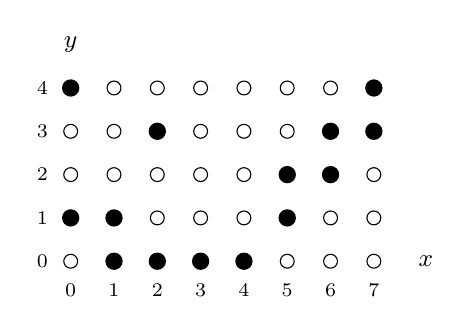
\begin{tikzpicture}[scale=0.55]
  \foreach \x in {0,...,7} \foreach \y in {0,...,4} \draw (\x,\y) circle (0.16);
  \foreach \p in {(0,1),(0,4),(1,0),(1,1),(2,0),(2,3),(3,0),(4,0),(5,1),(5,2),(6,2),(6,3),(7,3),(7,4)}
    \fill \p circle (0.2);
  \foreach \x in {0,...,7} \node[below] at (\x,-0.3) {\scriptsize $\x$};
  \foreach \y in {0,...,4} \node[left] at (-0.3,\y) {\scriptsize $\y$};
  \node at (8.2,0) {\small $x$};
  \node at (0,5.0) {\small $y$};
\end{tikzpicture}
\caption{The blackout $\Bs$ (filled) in $G_{5,8}=\{0,\dots,7\}\times\{0,\dots,4\}$.}\label{fig:witness}
\end{figure}

\section{Statement}\label{sec:statement}

\subsection*{Definitions}
Following the programs in the entry, the $n\times k$ grid is $\G=\{0,\dots,k-1\}\times\{0,\dots,n-1\}\subseteq\Z^2$. A \emph{rectangle} of $\G$ is a set $\{a,b,c,d\}$ where $a,b,c\in\G$ are pairwise distinct, $(a-b)\cdot(c-b)=0$, and $d=a+c-b\in\G$; let $\Rc_{n,k}$ be the set of rectangles. A set $B\subseteq\G$ is a \emph{valid blackout} if $R\mapsto R\setminus B$ is injective on $\Rc_{n,k}$, and $T(n,k)$ is the largest size of a valid blackout (the empty set is valid).
Here $d\notin\{a,b,c\}$: $d=a$ forces $c=b$, $d=c$ forces $a=b$, and $d=b$ gives $0=(a-b)\cdot(c-b)=-|a-b|^2$. So $a,b,c,d$ are the vertices, in cyclic order, of a non-degenerate rectangle with a right angle at $b$, and conversely every rectangle with vertices in $\G$ (axis-parallel or tilted, squares included) arises in this way.

\subsection*{The conjecture}
The conjecture is stated in the COMMENTS section of A397315 (entry by A.~Pemmasani, September~2, 2026; revision~\#38 of September~12, 2026), verbatim:
\begin{quote}
\texttt{Conjecture: T(n,m) = n+m whenever min(n,m) >= 4, except T(4,4) = 7 and T(4,5) = 8 (verified on seven cells through 6 X 6).}
\end{quote}
Since $T$ is symmetric (transpose the grid) and the entry lists $T(5,4)=8$, the exception $T(4,5)=8$ is read as covering $(5,4)$ as well.

\begin{conjecture}[Pemmasani \cite{A397315}]\label{conj}
For all $n,m$ with $\min(n,m)\ge4$: $T(4,4)=7$, $T(4,5)=T(5,4)=8$, and $T(n,m)=n+m$ otherwise.
\end{conjecture}

The cell $(5,8)$ is not exceptional, so under every reading of the exceptions the conjecture predicts $T(5,8)=13$.

\begin{theorem}\label{thm:main}
The set
\begin{align*}
  \Bs=\{&(0,1),(0,4),(1,0),(1,1),(2,0),(2,3),(3,0),\\
  &(4,0),(5,1),(5,2),(6,2),(6,3),(7,3),(7,4)\}
\end{align*}
is a valid blackout of $G_{5,8}$. Hence $T(5,8)\ge14>5+8$, and Conjecture~\ref{conj} is false.
\end{theorem}

\subsection*{Lean formalization}
The statement was formalized by math0 in \path{lean/Math0/Statements/OEIS/A397315.lean}, reviewed for fidelity, and frozen (SHA-256 \texttt{81afd722\ldots39eba61c5d}) before any proof attempt. The definitions on which \decl{statement} depends are, verbatim except that docstrings and blank lines are omitted:
\begin{lstlisting}
namespace Math0.Statements.A397315
def pt (n i : ℕ) : ℤ × ℤ := (((i / n : ℕ) : ℤ), ((i % n : ℕ) : ℤ))
def inGrid (n k : ℕ) (p : ℤ × ℤ) : Bool :=
  decide (0 ≤ p.1) && decide (p.1 < k) && decide (0 ≤ p.2) && decide (p.2 < n)
def idx (n : ℕ) (p : ℤ × ℤ) : ℕ := p.1.toNat * n + p.2.toNat
def rectMask? (n k a b c : ℕ) : Option ℕ :=
  let A := pt n a
  let B := pt n b
  let C := pt n c
  let D := A + C - B
  if a ≠ b ∧ b ≠ c ∧ a ≠ c ∧ (A.1 - B.1) * (C.1 - B.1) + (A.2 - B.2) * (C.2 - B.2) = 0 ∧
      inGrid n k D = true then
    some (2 ^ a ||| 2 ^ b ||| 2 ^ c ||| 2 ^ idx n D)
  else none
def rects (n k : ℕ) : List ℕ :=
  ((List.range (n * k)).flatMap fun a => (List.range (n * k)).flatMap fun b =>
    (List.range (n * k)).filterMap fun c => rectMask? n k a b c).eraseDups
def visible (R B : ℕ) : ℕ := Nat.xor R (Nat.land R B)
def notMem (x : ℕ) (l : List ℕ) : Bool := l.rec true fun y _ ih => !(Nat.beq x y) && ih
def pairwiseDistinct (l : List ℕ) : Bool := l.rec true fun x xs ih => notMem x xs && ih
def isValidBlackout (n k B : ℕ) : Bool := pairwiseDistinct ((rects n k).map (visible · B))
def card : ℕ → ℕ → ℕ
  | 0, _ => 0
  | len + 1, B => B % 2 + card len (B / 2)
def T (n k : ℕ) : ℕ :=
  ((List.range (2 ^ (n * k))).filter (isValidBlackout n k)).foldr
    (fun B m => max (card (n * k) B) m) 0
def statement : Prop :=
  ∀ n m : ℕ, 4 ≤ min n m →
    T n m = if n = 4 ∧ m = 4 then 7
      else if (n = 4 ∧ m = 5) ∨ (n = 5 ∧ m = 4) then 8
      else n + m
end Math0.Statements.A397315
\end{lstlisting}
\emph{Encoding.} The point $(x,y)\in\G$ has index $nx+y\in\{0,\dots,nk-1\}$, and \texttt{pt n i} $=(\lfloor i/n\rfloor, i\bmod n)$ inverts this numbering; a set $S$ of points is the bitmask $\sum_{(x,y)\in S}2^{nx+y}$. For indices $a,b,c$, \texttt{rectMask?} tests the conditions of the definition, with the dot product computed in $\Z$, and returns the mask of $\{a,b,c,d\}$. The list \texttt{rects n k} collects these masks over all ordered triples and erases duplicates (each rectangle arises from exactly $8$ triples: $b$ is any vertex and $a,c$ are its two neighbours, in either order), so it lists $\Rc_{n,k}$ once each. \texttt{visible R B} $=R\oplus(R\wedge B)$ is the mask of $R\setminus B$, and \texttt{pairwiseDistinct} decides \texttt{List.Nodup} (Lemma~\ref{lem:pd}), so \texttt{isValidBlackout n k B} says that $B$ is a valid blackout. \texttt{card (n*k) B} counts the $1$ bits of $B$ below position $nk$, and \texttt{T n k} maximizes it over the valid masks $B<2^{nk}$; this is $T(n,k)$, and \decl{statement} is Conjecture~\ref{conj}.

\emph{Check against the OEIS data.} The statement file also defines the antidiagonal reading order \texttt{cell} and the sequence \texttt{a} with the entry's offset~$2$. Ten theorems \texttt{T\_2\_2}, \dots, \texttt{T\_5\_2}, each proved by \texttt{decide +kernel}, evaluate $T$ from the definition on the first ten cells (at most $2^{12}$ candidate blackouts each), and \decl{a_data} assembles them: the terms $4,4,4,5,5,5,6,6,6,6$ agree with the entry. During formalization and fidelity review, Python transcriptions of the same encoding reproduced the first $15$ listed terms (among them $T(4,4)=7$) and $T(4,5)=T(5,4)=8$, and a referee's exact MaxSAT computation reproduced $13$ listed values, among them $T(5,5)=10$, $T(6,6)=12$ and $T(5,7)=12$.

\section{Proof}\label{sec:proof}

The proof follows \path{lean/Math0/Frontier/OEIS/A397315.lean}; names of private auxiliary declarations are given in brackets. Throughout, $n=5$, $k=8$, and points are identified with their indices $0,\dots,39$. In indices, the blackout and its mask [\texttt{Bw}] are
\[
  \Bs=\{1,4,5,6,10,13,15,20,26,27,32,33,38,39\},\qquad B_w=\textstyle\sum_{i\in\Bs}2^i=837721039986<2^{40}.
\]
Evaluating \texttt{isValidBlackout 5 8 Bw} directly in the kernel exhausts memory (evaluating \texttt{rectMask?} alone on the $40^3$ triples took about $219$\,s and $3.9$\,GB). The proof therefore replaces \texttt{rectMask?} by a natural-number version and splits the check into a covering step and an injectivity step.

\begin{lemma}[\decl{rectMask_eq}]\label{lem:fast}
For $i\in\N$ write $i_x=\lfloor i/n\rfloor$, $i_y=i\bmod n$, and let $\dot-$ be truncated subtraction. For all $n,k,a,b,c\in\N$, \texttt{rectMask?\ n k a b c} equals \texttt{fastMask n k a b c}, defined as \texttt{some}$(2^a\mid 2^b\mid 2^c\mid 2^{\delta})$, $\delta=(a_x+c_x\dot-b_x)\,n+(a_y+c_y\dot-b_y)$, if $a,b,c$ are pairwise distinct and
\begin{gather}
  a_xc_x+b_x^2+a_yc_y+b_y^2=a_xb_x+b_xc_x+a_yb_y+b_yc_y,\label{eq:dot}\\
  b_x\le a_x+c_x<k+b_x,\qquad b_y\le a_y+c_y<n+b_y,\label{eq:grid}
\end{gather}
and \texttt{none} otherwise ($\mid$ is bitwise or).
\end{lemma}

\begin{proof}
In \texttt{rectMask?}, $A=(a_x,a_y)$, $B=(b_x,b_y)$, $C=(c_x,c_y)\in\Z^2$. The expression $(a_x-b_x)(c_x-b_x)+(a_y-b_y)(c_y-b_y)$ is the left side of \eqref{eq:dot} minus its right side, so it vanishes in $\Z$ if and only if \eqref{eq:dot} holds in $\N$ (\texttt{linear\_combination} and injectivity of $\N\to\Z$). The point $D=(a_x+c_x-b_x,\,a_y+c_y-b_y)$ is in the grid if and only if \eqref{eq:grid} holds, and then its coordinates are nonnegative, so \texttt{toNat} agrees with truncated subtraction and \texttt{idx n D} $=\delta$ (\texttt{omega}).
\end{proof}

Let $\Lr$ [\texttt{Lr}] be the explicit sorted list of $364$ numbers in the proof file, from $99=2^0+2^1+2^5+2^6$ (the unit square at the origin) to $850403524608$.

\begin{lemma}[\decl{chk_0}--\decl{chk_39}, \decl{F_true}, \decl{mem_rects}]\label{lem:cover}
Every element of \texttt{rects 5 8} belongs to $\Lr$.
\end{lemma}

\begin{proof}
Let $F(a,b,c)$ [\texttt{F}] be \texttt{true} if \texttt{fastMask 5 8 a b c} is \texttt{none}, and otherwise, if it is \texttt{some r}, the result of a linear scan of $\Lr$ for $r$ by \texttt{Nat.beq} [\texttt{scan}, \texttt{memL}]. Let $\mathrm{chkA}(a)=\bigwedge_{b<40}\bigwedge_{c<40}F(a,b,c)$, written as two nested \texttt{Nat.rec} loops [\texttt{chkA}].
For each $a<40$, the theorem \texttt{chk\_a : chkA a = true} is proved by \texttt{decide +kernel}: the kernel evaluates $F(a,b,c)$ for the $1600$ pairs $(b,c)$ and reduces $\mathrm{chkA}(a)$ to \texttt{true}. Altogether this covers the $64000$ triples, of which $2912=8\cdot364$ yield a mask and trigger a scan of $\Lr$.
By induction on $m$, if the loop \texttt{Nat.rec true (fun c ih => f c \&\& ih) m} evaluates to \texttt{true}, then $f(c)=\texttt{true}$ for all $c<m$ [\decl{loop_spec}]; applied twice, with \texttt{interval\_cases} on $a$ [\decl{chk_all}], this gives $F(a,b,c)=\texttt{true}$ for all $a,b,c<40$. A successful scan implies membership, by induction on the list [\decl{mem_of_scan}].
Now let $r\in\texttt{rects 5 8}$. Every element of $l.\texttt{eraseDups}$ lies in $l$, so \texttt{rectMask?\ 5 8 a b c = some r} for some $a,b,c<40$. By Lemma~\ref{lem:fast}, \texttt{fastMask 5 8 a b c = some r}, and $F(a,b,c)=\texttt{true}$ says that $r\in\Lr$.
\end{proof}

Only the inclusion is used, but $\Lr$ is exactly the set of rectangle masks of $G_{5,8}$ (Python computations by math0 and a referee, who also obtained $364$ rectangles from the entry's own program); $280=\binom82\binom52$ of them are axis-parallel and $84$ are tilted.

\begin{lemma}[\decl{dist}]\label{lem:dist}
\texttt{pairwiseDistinct (Lr.map (visible · Bw)) = true}: the $364$ masks of $R\setminus\Bs$, $R\in\Lr$, are pairwise distinct.
\end{lemma}

\begin{proof}
A closed Boolean computation, proved by \texttt{decide +kernel}: the kernel computes the masks $R\oplus(R\wedge B_w)$ and makes the $\binom{364}{2}=66066$ comparisons by \texttt{Nat.beq}, all returning \texttt{false}.
\end{proof}

\begin{lemma}[\decl{pd_iff}, \decl{nodup_eraseDups'}]\label{lem:pd}
For lists $l$ of natural numbers, $\texttt{pairwiseDistinct}\ l=\texttt{true}$ if and only if $l$ has no duplicates, and $l.\texttt{eraseDups}$ has no duplicates.
\end{lemma}

\begin{proof}
The first claim follows by induction on $l$ from $\texttt{notMem}\ x\ l=\texttt{true}\iff x\notin l$ [\decl{notMem_iff}], itself proved by induction using $\texttt{Nat.beq}\ x\ y=\texttt{true}\iff x=y$. For the second, use strong induction on the length: $(x::xs).\texttt{eraseDups}=x::(xs.\texttt{filter}(\cdot\ne x)).\texttt{eraseDups}$, the head does not occur in the tail, and the filtered list is shorter.
\end{proof}

\begin{proposition}[\decl{valid}]\label{prop:valid}
\texttt{isValidBlackout 5 8 Bw = true}; that is, $\Bs$ is a valid blackout of $G_{5,8}$.
\end{proposition}

\begin{proof}
By Lemma~\ref{lem:pd} we must show that \texttt{(rects 5 8).map (visible · Bw)} has no duplicates. The list \texttt{rects 5 8} has none (Lemma~\ref{lem:pd}). By Lemmas~\ref{lem:dist} and~\ref{lem:pd}, $R\mapsto\texttt{visible}(R,B_w)$ is injective on the elements of $\Lr$, hence, by Lemma~\ref{lem:cover}, on those of \texttt{rects 5 8}; the image of a duplicate-free list under a map injective on its elements is duplicate-free (\texttt{List.Nodup.map\_on}).
\end{proof}

\subsection*{Proof of Theorem~\ref{thm:main}}
The kernel checks \texttt{card (5 * 8) Bw = 14} by \texttt{decide +kernel} [\decl{card_Bw}], and $B_w<2^{40}$ holds by \texttt{norm\_num}. With Proposition~\ref{prop:valid}, $B_w$ belongs to the list $(\texttt{List.range}\ 2^{40}).\texttt{filter}(\texttt{isValidBlackout 5 8})$ whose \texttt{foldr} of \texttt{max} defines \texttt{T 5 8}; such a fold is at least its value at each element [\decl{le_foldr}], so $14\le\texttt{T 5 8}$ [\decl{T_5_8_ge}].
Assume \decl{statement}. Since $\min(5,8)\ge4$ and neither exception applies, it gives $\texttt{T 5 8}=5+8=13$, a contradiction:
\begin{lstlisting}
theorem result : ¬ statement := by
  intro h
  have h58 := h 5 8 (by norm_num)
  have h14 := T_5_8_ge
  rw [h58] at h14
  norm_num at h14
\end{lstlisting}
\qed

\subsection*{A check with fewer comparisons (not formalized)}
Any three vertices of a rectangle are a vertex $v$ and its two neighbours $u,w$, forming a right triangle with its unique right angle at $v$; so they determine the rectangle (the fourth vertex is $u+w-v$). Hence two distinct rectangles can have the same visible set only if it has at most two points, and $B$ is valid if and only if at most one rectangle lies in $B$, no two rectangles with exactly three vertices in $B$ share their visible vertex, and no two with exactly two vertices in $B$ share their visible pair. For $\Bs$ the numbers of rectangles with $0,1,2,3,4$ vertices in $\Bs$ are $53,148,139,24,0$, and the $24$ visible points and $139$ visible pairs are pairwise distinct (Python computation). Adding any of the $26$ points of $G_{5,8}\setminus\Bs$ to $\Bs$ gives an invalid blackout, so $\Bs$ is maximal under inclusion.

\begin{remark}[Further values; not formalized]
The math0 SAT computations (CaDiCaL) and a referee's MaxSAT computation give $T(5,8)=14$ exactly, in agreement with Pemmasani's \texttt{kfvalue\_5\_8} \cite{Pem}. The SAT computations also found valid blackouts showing $T(5,m)\ge m+6$ for $9\le m\le12$, consistent with Pemmasani's $f(5,m)=m+6$, and report $T(4,m)=m+4$ for $9\le m\le11$, $T(6,7)=13$, and $T(3,m)=m+2$ for $3\le m\le25$.
\end{remark}

\section{Machine verification}\label{sec:lean}

\subsection*{Files and declarations}
The proof is in \path{lean/Math0/Frontier/OEIS/A397315.lean} of the math0 repository, \url{https://github.com/Foundation-0/math0}. The main theorem is \decl{Math0.Frontier.A397315.result}, of type \texttt{¬ Math0.Statements.A397315.statement}. The proof file contains no \texttt{sorry}, \texttt{admit}, \texttt{native\_decide}, \texttt{axiom} or \texttt{set\_option} (the statement file sets \texttt{maxRecDepth} for four data checks).

\subsection*{Kernel computation}
The finite computations are the $40$ checks \texttt{chk\_0}, \dots, \texttt{chk\_39}, \decl{dist} and \decl{card_Bw}, all by \texttt{decide +kernel}: the kernel reduces the Boolean to \texttt{true} while type-checking the proof term, using its built-in arithmetic on natural-number literals. No compiled code is trusted, unlike with \texttt{native\_decide}, which would add the axiom \decl{Lean.ofReduceBool}. The file compiles in about $60$ to $95$\,s with peak memory about $2.5$\,GB.

\subsection*{Audit}
The file ends with \texttt{\#math0\_settles} \decl{Math0.Frontier.A397315.result} \decl{Math0.Statements.A397315.statement}. This command (\path{lean/Math0/Audit.lean}) fails unless (1) \decl{statement} is a definition of type \texttt{Prop} without universe parameters; (2) \decl{statement} and \decl{result} depend on no axioms besides \decl{propext}, \decl{Classical.choice} and \decl{Quot.sound}, which rejects \decl{sorryAx}, the axioms \decl{Lean.ofReduceBool} and \decl{Lean.trustCompiler} of \texttt{native\_decide}, and custom axioms; and (3) the type of \decl{result} is syntactically the statement or its negation, up to metadata and with no unfolding. Running \texttt{lake env lean} on the file (in \path{lean}) reports
\begin{lstlisting}
math0 audit: 'Math0.Statements.A397315.statement' depends on axioms [propext]
math0 audit: 'Math0.Frontier.A397315.result' depends on axioms
  [Classical.choice, Quot.sound, propext]
math0 statement check: 'Math0.Frontier.A397315.result' refutes
  'Math0.Statements.A397315.statement'
\end{lstlisting}

\subsection*{Toolchain and reproduction}
We use Lean~4 \cite{Lean4} \texttt{v4.33.1} and Mathlib \cite{Mathlib} \texttt{v4.33.1}, pinned in \path{lean/}; the repository also pins formal-conjectures \cite{FC} at commit \texttt{c77fdd4}, which this result does not use.
To reproduce, run \path{scripts/verify.sh} from the repository root: it builds all math0 results with \texttt{lake build}, re-running every audit command, and checks that the pinned dependencies are unmodified.

\begin{thebibliography}{99}
\small

\bibitem{FC}
M.~Firsching, P.~Lezeau, S.~Mercuri, M.~Z. Horv\'ath, Y.~Dillies, C.~S\"onne, E.~Wieser, F.~Zhang, T.~Hubert, B.~Ag\"uera y Arcas, and P.~Kohli, \emph{Formal Conjectures: An open and evolving benchmark for verified discovery in mathematics}, arXiv:2605.13171, 2026. Repository: \url{https://github.com/google-deepmind/formal-conjectures}.

\bibitem{Kagey}
P.~Kagey, \emph{Open Problem Collection, Problem 001}, \url{https://peterkagey.com/problems/001/}.

\bibitem{Mathlib}
The mathlib Community, \emph{The Lean mathematical library}, in: Proceedings of the 9th ACM SIGPLAN International Conference on Certified Programs and Proofs (CPP 2020), ACM, 2020, 367--381.

\bibitem{Lean4}
L.~de Moura and S.~Ullrich, \emph{The Lean 4 theorem prover and programming language}, in: Automated Deduction -- CADE 28, Lecture Notes in Comput. Sci. \textbf{12699}, Springer, 2021, 625--635.

\bibitem{A397315}
The OEIS Foundation Inc., \url{https://oeis.org/A397315}, entry by A.~Pemmasani (2026).

\bibitem{A399580}
The OEIS Foundation Inc., \url{https://oeis.org/A399580}, entry by A.~Pemmasani (2026).

\bibitem{Pem}
A.~Pemmasani, \emph{Solvers, exhaustive verification, and pre-registration ledger for Problem 001}, GitHub repository \url{https://github.com/apemm/Kagey-Problems} (commits \texttt{45b175b}, October~17, 2026, and \texttt{8df4162} and \texttt{a46acfd}, October~18, 2026).

\end{thebibliography}
\end{document}
